\chapter{Methodology}
\label{chap:methodology}

This chapter describes our pipeline for analyzing the topology of neural network decision 
boundaries. For a given neural network and dataset, our pipeline consists of the
following steps:
\begin{enumerate}
    \item Sample a subset of the dataset and obtain model predictions on this subset
    \item Construct the LVR complex using the predicted labels
    \item Construct the LVR complex using ground truth labels
    \item Compare the resulting persistence diagrams using topological metrics
\end{enumerate}
We first present the datasets used in our experiments, including both synthetic 2D data 
for interpretable validation and real-world image datasets. We then detail the neural 
network architectures used for classification. Finally, we describe our choices for the 
key components of the pipeline: the construction of the Labeled Vietoris-Rips complex 
for both binary and multiclass settings, and the metrics used for comparing persistence 
diagrams.

\section{Datasets and models}

To evaluate our approach we have used the MNIST~\cite{deng2012mnist}, FashionMNIST~\cite{xiao2017fashionmnistnovelimagedataset}
and CIFAR10~\cite{krizhevsky2009learning} datasets with the predefined training and testing splits.
These datasets are commonly used as simple problems, providing a robust foundation for evaluating model performance.
Additionally, we have also used synthetic 2D binary classification datasets for more easily interpretable experiments.
In the 2D setting, we can visualize the simplicial complex, as well as know the ground truth decision boundary
and its homology groups. For subsampling, we use 2000 points unless specified otherwise.

The synthetic datasets consist of points uniformly sampled from the $[ - 1, 1]^2$ square,
with a total of $2000$ points per dataset. Figure~\ref{fig:synthetic-datasets-2d}
shows the two datasets used. The nested annuli dataset, also referred to as simply the nested dataset,
has the decision boundary of 5 concentric circles, with the $i$-th circle having the radius of $0.18 \cdot (i + 1)$.
The manyholes dataset assigns a point $(x, y)$ class 1 if
\begin{equation}
    \sin(10x) + \sin(10y) - x - y > 0,
\end{equation}
and class 0 otherwise. This results in multiple ``holes'' in the decision boundary at various scales.

% The synthetic datasets are shown in Figure~\ref{fig:synthetic-datasets-2d}.
% with each dataset consisting of $10000$ points, uniformly sampled from $[ - 1, 1]^2$
% and split into training and testing sets with a ratio of $0.8:0.2$.

\begin{figure}
    \centering
    \begin{subfigure}{0.49\textwidth}
        \includegraphics[width=\textwidth]{plots/nested.jpg}
        \caption{The nested annuli dataset}
    \end{subfigure}
    \begin{subfigure}{0.49\textwidth}
        \includegraphics[width=\textwidth]{plots/manyholes.jpg}
        \caption{The manyholes dataset}
    \end{subfigure}
    % \begin{subfigure}{0.45\textwidth}
    %     \resizebox{\textwidth}{!}{
    %         \begin{tikzpicture}
    %             \begin{axis}[
    %                 enlargelimits=false,
    %             ]
    %             \addplot+[
    %                 only marks,
    %                 scatter,
    %                 mark size=2pt,
    %                 scatter src=explicit]
    %             table[meta=class]
    %             {data/2d/manyholes.dat};
    %             \end{axis}
    %         \end{tikzpicture}
    %     }
    %     \caption{Many holes dataset}
    % \end{subfigure}
    % \begin{subfigure}{0.45\textwidth}
    %     \resizebox{\textwidth}{!}{
    %         \begin{tikzpicture}
    %             \begin{axis}[
    %                 enlargelimits=false,
    %             ]
    %             \addplot+[
    %                 only marks,
    %                 scatter,
    %                 mark size=2pt,
    %                 scatter src=explicit]
    %             table[meta=class]
    %             {data/2d/nested.dat};
    %             \end{axis}
    %         \end{tikzpicture}
    %     }
    %     \caption{Nested annuli dataset}
    % \end{subfigure}
    \caption{Synthetic 2D datasets}
    \label{fig:synthetic-datasets-2d}
\end{figure}


% \todo{Maybe add 3D}

For the image datasets, we have used the following models:
\begin{enumerate}
    \item \emph{FC}: A fully connected neural network with layer sizes
    $w \cdot h, 512, 128, 16, 10$, where $w$ and $h$ are input image width and height.
    The network uses ReLU activations after each layer, and a softmax activation after the last layer.
    \item \emph{CNN}: A convolutional neural network with the architecture given in the PyTorch MNIST example\footnote{
        Available at \href{https://github.com/pytorch/examples/tree/main/mnist}{https://github.com/pytorch/examples/tree/main/mnist}.
    },
    with the following parameters added:
    \begin{enumerate}
        \item \verb|in_size| and \verb|in_channels|: To account for CIFAR-10 having 3 channels and $32 \times 32$ images,
        as opposed to 1 channel and $28 \times 28$ images in MNIST and FashionMNIST,
        \verb|in_channels| sets the number of input channels, and \verb|in_size|
        adjusts the number of neurons in the first fully connected layer.
        \item \verb|scale|: A multiplicative factor for the number of convolutional filters and number of neurons in the fully connected layers.
        \item \verb|extra_cnn|: Adds convolutional layers with $64 \cdot \verb|scale|$ channels, a $3 \times 3$ kernel size,
        1-pixel padding and stride, as well as a ReLU activation.
        \item \verb|extra_linear|: Adds fully connected layers with $128 \cdot \verb|scale|$ neurons,
        as well as a ReLU activation.
    \end{enumerate}
\end{enumerate}

\section{Metrics and evaluation}

For estimating similarity between two persistence diagrams,
we use the following metrics:

\begin{definition}
    For \(q \geq 1\), the \emph{Wasserstein distance} between two persistence diagrams
    $\dgm_p(\mathcal{F})$ and $\dgm_p(\mathcal{G})$ is defined as
    \begin{equation}
        d_{W, q}(\dgm_p(\mathcal{F}), \dgm_p(\mathcal{G}))
        = \left[\inf_{\pi \in \Pi} \left(\sum_{x \in \dgm_p(\mathcal{F})}
        \norm{x - \pi(x)}_{\infty}^q\right)\right]^{1 / q}
    \end{equation}
\end{definition}

\begin{definition}
    The \emph{total bar length} (TBL) of a persistence diagram $\dgm_p(\mathcal{F})$ is defined as
    \begin{equation}
        \sum_{(b, d) \in \dgm_p(\mathcal{F})} d - b
    \end{equation}
\end{definition}

The Wasserstein distance and TBL offer different approaches to comparing
persistence diagrams. The Wasserstein distance directly measures the similarity
between two persistence diagrams by comparing them to each other. In contrast,
total bar length is a single-diagram measure that quantifies the complexity of
an individual persistence diagram. To compare two diagrams using TBL, we
calculate the TBL for each diagram separately and then take the absolute
difference between these two values.

\section{Simplicial complex}
\label{sec:complex}

% \begin{itemize}
    % \item Labeled Vietoris-Rips complex
    % \item Usage of \texttt{ripser++} and \texttt{giotto-ph}
    % \item Generalization to multiclass classification
%     \item Circumcircle filtering (show why it's needed in 2D, but not in high-dim)
%     \item Dowker complex
% \end{itemize}

We use the labeled Vietoris-Rips complex, as presented in previous research~\cite{ramamurthy2018topologicaldataanalysisdecision}.
To improve computational performance, we used the \verb|ripser++|~\cite{zhang2020gpu}
and the \verb|giotto-ph|~\cite{burella2021giottoph} packages for computing Vietoris-Rips persistence barcodes.
Both of these methods outperform the original \verb|ripser|~\cite{Bauer2021Ripser} package in terms of runtime.
Due to GPU memory limitations, we use \verb|giotto-ph| in all experiments.

In previous research~\cite{li2020finding,ramamurthy2018topologicaldataanalysisdecision},
classification datasets with \(n > 2\) classes were split into
\(\binom{n}{2}\) binary classification problems.
However, this process loses topological information, as shown in an example dataset in Figure~\ref{fig:binarization}.
The decision boundary for all three clsases (\ref{fig:binarization:all})
has a non-trivial first homology group \(H_1\), but
this is not the case for any binary classification problem for this dataset
(\ref{fig:binarization:rg}, \ref{fig:binarization:gb}).
Moreover, the decision boundary is disconnected for the red and green subdataset,
but connected for the full dataset.

\begin{figure}
    \centering
    \begin{subfigure}[b]{0.3\textwidth}
        \centering
        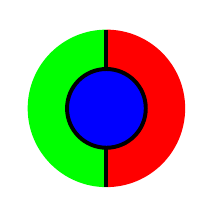
\begin{tikzpicture}
            \fill[blue] (0,0) circle(0.5);
    
            \fill[red]
            (0,-0.5)           % Start at bottom inner point
            arc(-90:90:0.5)     % Inner arc: radius=0.5 from -90° to 90° (bottom to top on the right side)
            -- (0,1)            % Line from top inner (0,0.5) to top outer (0,1)
            arc(90:-90:1)       % Outer arc: radius=1 from 90° to -90° (top to bottom on the right side)
            -- cycle;           

            \begin{scope}[rotate=180]
            \fill[green]
            (0,-0.5)
            arc(-90:90:0.5)
            -- (0,1)
            arc(90:-90:1)
            -- cycle;
            \end{scope}
            
            % Decision boundary
            \draw[line width=0.5mm] (0, 0.5) -- (0, 1);
            \draw[line width=0.5mm] (0, -0.5) -- (0, -1);
            \draw[line width=0.5mm] (0,0) circle (0.5);
        \end{tikzpicture}
        \caption{All classes shown}
        \label{fig:binarization:all}
    \end{subfigure}
    \begin{subfigure}[b]{0.3\textwidth}
        \centering
        
\begin{tikzpicture}
            \fill[red]
            (0,-0.5)           % Start at bottom inner point
            arc(-90:90:0.5)     % Inner arc: radius=0.5 from -90° to 90° (bottom to top on the right side)
            -- (0,1)            % Line from top inner (0,0.5) to top outer (0,1)
            arc(90:-90:1)       % Outer arc: radius=1 from 90° to -90° (top to bottom on the right side)
            -- cycle;           

            \begin{scope}[rotate=180]
            \fill[green]
            (0,-0.5)
            arc(-90:90:0.5)
            -- (0,1)
            arc(90:-90:1)
            -- cycle;
            \end{scope}
            
            % Decision boundary
            \draw[line width=0.5mm] (0, 0.5) -- (0, 1);
            \draw[line width=0.5mm] (0, -0.5) -- (0, -1);
        \end{tikzpicture}
        \caption{Red and green classes}
        \label{fig:binarization:rg}
    \end{subfigure}
    \begin{subfigure}[b]{0.3\textwidth}
        \centering
        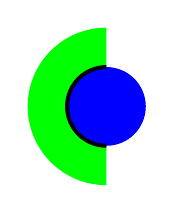
\begin{tikzpicture}
            \fill[blue] (0,0) circle(0.5);
    
            \begin{scope}[rotate=180]
            \fill[green]
            (0,-0.5)
            arc(-90:90:0.5)
            -- (0,1)
            arc(90:-90:1)
            -- cycle;
            \end{scope}
            
            % Decision boundary
            \draw[line width=0.5mm] (0,0.5) arc (90:270:0.5);
        \end{tikzpicture}
        \caption{Green and blue classes}
        \label{fig:binarization:gb}
    \end{subfigure}
    \caption{A 2D example that demonstrates the loss of topological information when binarizing a multiclass dataset.
    Red, green and blue shapes denote different classes, the black line is the decision boundary.}
    \label{fig:binarization}
\end{figure}

To avoid this information loss, we propose applying the Labeled Vietoris-Rips complex
to multiclass classification problems. The construction of the complex is exactly the same
as in the binary setting, with neighbors of different classes being connected and 2-hop
neighbors being connected afterwards. Notably, the labeled \v{C}ech complex cannot be
applied to the multiclass setting without modifications, as it uses elements of only one
class as its vertices.

Consistent with previous research, we only consider $0$ and $1$-dimensional homology groups,
and thus only compute simplices up to dimension $3$. Unless specified otherwise, all homology
groups and persistence diagrams discussed are in dimension $1$.
